\documentclass[a4paper,10pt,reqno]{amsart}

\usepackage[utf8]{inputenc}
\usepackage[foot]{amsaddr}
\usepackage{amsmath,amsfonts,amssymb,amsthm,mathrsfs,bm}
\usepackage[margin=0.95in]{geometry}
\usepackage{color}
\usepackage[dvipsnames]{xcolor}

\input{toc-config.tex}

\usepackage{mathtools,enumerate,mathrsfs,graphicx}
\usepackage{epstopdf}
\usepackage{hyperref}

\usepackage{latexsym}


\definecolor{CommentGreen}{rgb}{0.0,0.4,0.0}
\definecolor{Background}{rgb}{0.9,1.0,0.85}
\definecolor{lrow}{rgb}{0.914,0.918,0.922}
\definecolor{drow}{rgb}{0.725,0.745,0.769}

\usepackage{listings}
\usepackage{textcomp}
\usepackage{gensymb}
\lstloadlanguages{Matlab}%
\lstset{
    language=Matlab,
    upquote=true, frame=single,
    basicstyle=\small\ttfamily,
    backgroundcolor=\color{Background},
    keywordstyle=[1]\color{blue}\bfseries,
    keywordstyle=[2]\color{purple},
    keywordstyle=[3]\color{black}\bfseries,
    identifierstyle=,
    commentstyle=\usefont{T1}{pcr}{m}{sl}\color{CommentGreen}\small,
    stringstyle=\color{purple},
    showstringspaces=false, tabsize=5,
    morekeywords={properties,methods,classdef},
    morekeywords=[2]{handle},
    morecomment=[l][\color{blue}]{...},
    numbers=none, firstnumber=1,
    numberstyle=\tiny\color{blue},
    stepnumber=1, xleftmargin=10pt, xrightmargin=10pt
}

\numberwithin{equation}{section}
\synctex=1

\hypersetup{
    unicode=false, pdftoolbar=true, 
    pdfmenubar=true, pdffitwindow=false, pdfstartview={FitH}, 
    pdftitle={ELE2024 Coursework}, pdfauthor={A. Author},
    pdfsubject={ELE2024 coursework}, pdfcreator={A. Author},
    pdfproducer={ELE2024}, pdfnewwindow=true,
    colorlinks=true, linkcolor=red,
    citecolor=blue, filecolor=magenta, urlcolor=cyan
}


% CUSTOM COMMANDS
\renewcommand{\Re}{\mathbf{re}}
\renewcommand{\Im}{\mathbf{im}}
\newcommand{\R}{\mathbb{R}}
\newcommand{\N}{\mathbb{N}}
\newcommand{\C}{\mathbb{C}}
\newcommand{\lap}{\mathscr{L}}
\newcommand{\dd}{\mathrm{d}}
\newcommand{\smallmat}[1]{\left[ \begin{smallmatrix}#1 \end{smallmatrix} \right]}

%opening
\title[ELE2024 Lab 1]{Lab report for the ELE2024 Lab 1}

\author[D. Lim]{David Lim}

\address[D. Lim]{. Email addresses: \href{mailto:dlim04@qub.ac.uk}{dlim04@qub.ac.uk}}
% \thanks{Some note goes here. 
%        Version 0.0.1. Last updated:~\today.}
\begin{document}

\maketitle

The code for this lab can be found \href{https://github.com/drlim2u/Lane-Keeping}{here}.

\section{Question 1}\label{sec:q1}
    Simulate the open-loop trajectory of the vehicle over \(t \in [0, 2]\) with a constant steering action, \(u(t) = 2\degree\) (in the clockwise direction), starting from the initial state \(x(0) = 0, y(0) = 30 cm, \theta(0) = 5\degree\).

    \subsection{Question 1.1}
    Plot \(x(t), y(t)\) and \(\theta(t)\) again time in three separate figures.
    \begin{figure}[h]
        \centering
        \includegraphics[width=0.6\linewidth]{figures/question_1_1_a.eps}
        \caption{A plot of the simulation of the vehicle with the x position of the vehicle in respect to time.}
    \end{figure}

    \begin{figure}[h]
        \centering
        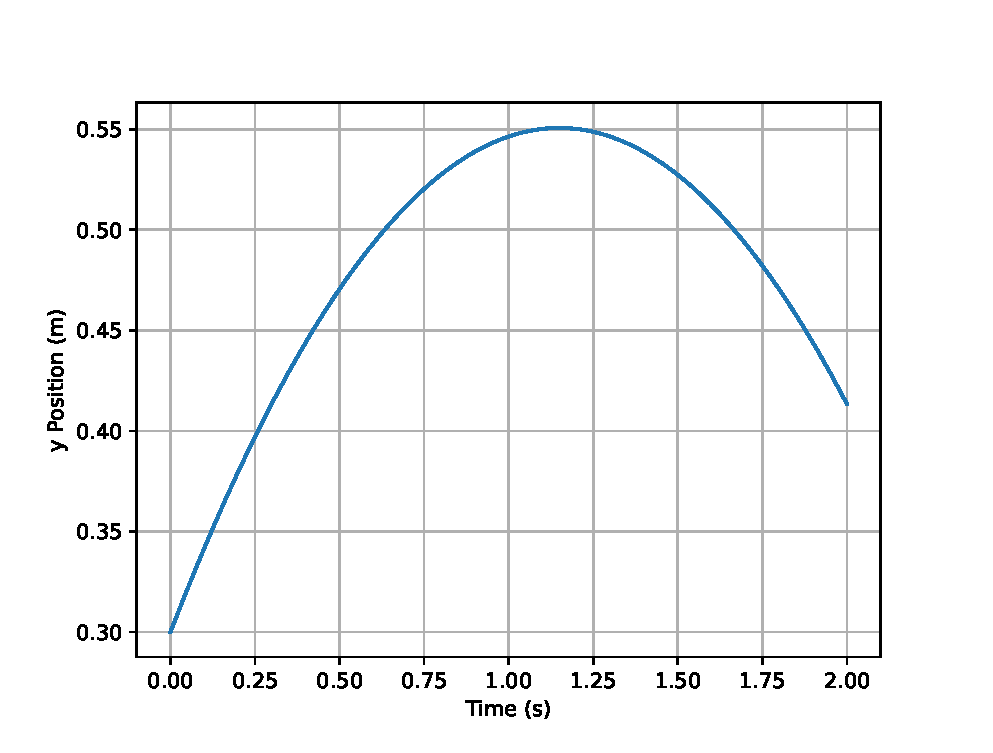
\includegraphics[width=0.6\linewidth]{figures/question_1_1_b.eps}
        \caption{A plot of the simulation of the vehicle with the y position of the vehicle in respect to time.}
    \end{figure}

    \begin{figure}[h]
        \centering
        \includegraphics[width=0.6\linewidth]{figures/question_1_1_c.eps}
        \caption{A plot of the simulation of the vehicle with the theta of the vehicle in respect to time.}
    \end{figure}
    
    \clearpage
    
    \subsection{Question 1.2}
    Plot the trajectory of the vehicle on the x - y plane.
    
    \begin{figure}[h]
        \centering
        \includegraphics[width=0.6\linewidth]{figures/question_1_2.eps}
        \caption{A plot of the simulation of the vehicle with the y position of the vehicle in respect to the x position of the vehicle.}
    \end{figure}
    
\clearpage
    
\section{Question 2}\label{sec:q2}
Suppose that the system input is subjected to a constant additive disturbance with \(w(t) = 1\degree\) for all \(t \geq 0\) and the sampling rate is 40 Hz.

    \subsection{Question 2.1}
        Suppose that the system is controlled with a P controller. Plot in the same axes the \((x, y)\) trajectories of the system for \(t \in [0, 50]\) for different values of \(K_p\) (starting from some initial point).
        
        \begin{figure}[h]
            \centering
            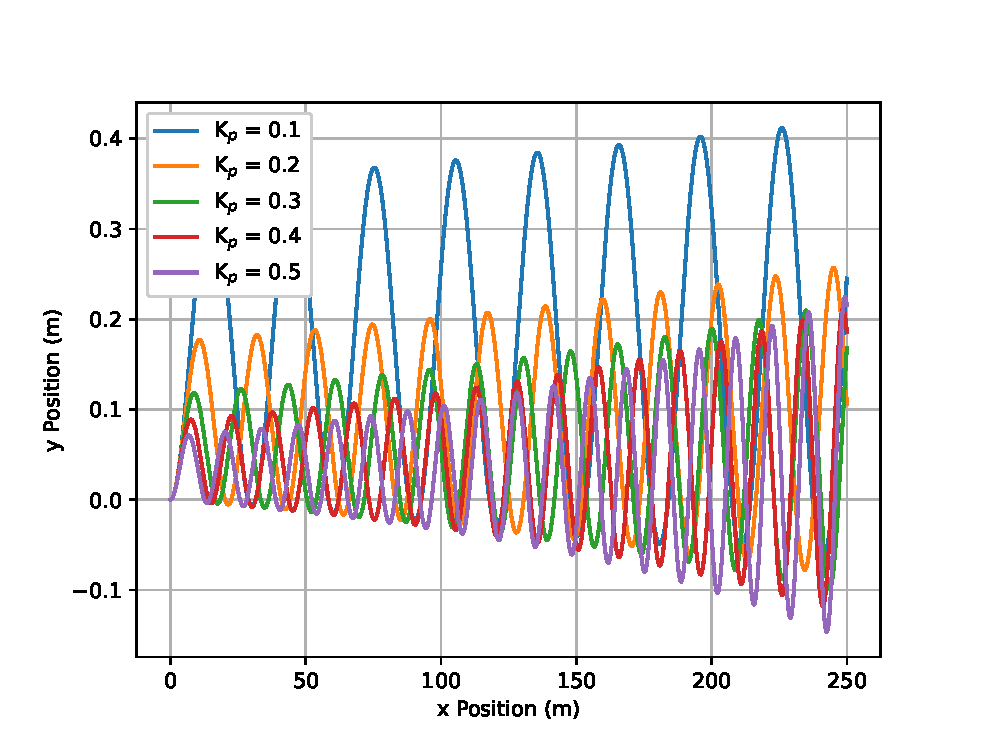
\includegraphics[width=0.6\linewidth]{figures/question_2_1.eps}
            \caption{A plot of the simulation of the vehicle with the y position of the vehicle in respect to the x position with varying proportionality constants.}
        \end{figure}
        
        \medskip
        As shown in Figure 5 increasing the magnitude of the \(K_p\) increases the frequency of the oscillations measured within the system. Furthermore, as \(K_p\) increases the initial magnitude of the oscillations decrease however, increasing \(K_p\) increases the rate of change of the magnitude of the oscillations of the car increases with respect to time. It also reduces the impact of the additive disturbance.
        
    \subsection{Question 2.2}
         Suppose that the system is controlled with a PD controller. Fix the value of \(K_p\) and plot in the same axes the (x, y) trajectory of the system for \(t \in [0, 50]\) for different values of \(K_d\).
         
         \begin{figure}[h]
            \centering
            \includegraphics[width=0.6\linewidth]{figures/question_2_2.eps}
            \caption{A plot of the simulation of the vehicle with the y position of the vehicle in respect to the x position of the vehicle with varying differential constants.}
        \end{figure}
        
        \medskip
        As shown in figure 6 as the \(K_d\) is increased the time it takes for the y position to reach equilibrium also increases. However, increasing \(K_d\) also reduces the number of oscillations that occur, therefore improving the stability of the system.
        
    \subsection{Question 2.3}
        Determine a triple of PID parameters so that the closed-loop system behaves “nicely,” i.e., it converges fast to the set point without a constant bias and does not exhibit oscillations. Using the triple of \(K_p\), \(K_d\) and \(K_i\) you chose, produce two plots: (i) u(t) vs time, (ii) the (x, y) trajectory of the system, for \(t \in [0, 50]\).
        
        \medskip
        For this question the values were chosen such that \(K_p = 0.4, K_d = 0.5\) and \(K_i = 0.1\). The initial state of the vehicle was \(x(0) = 0, y(0) = 0, \theta(0) = 0\).
        
        \begin{figure}[h]
            \centering
            \includegraphics[width=0.6\linewidth]{figures/question_2_3_a.eps}
            \caption{A plot of the simulation of the vehicle with the y position of the vehicle in respect to the x position with varying differential constants.}
        \end{figure}
        
        \begin{figure}[h]
            \centering
            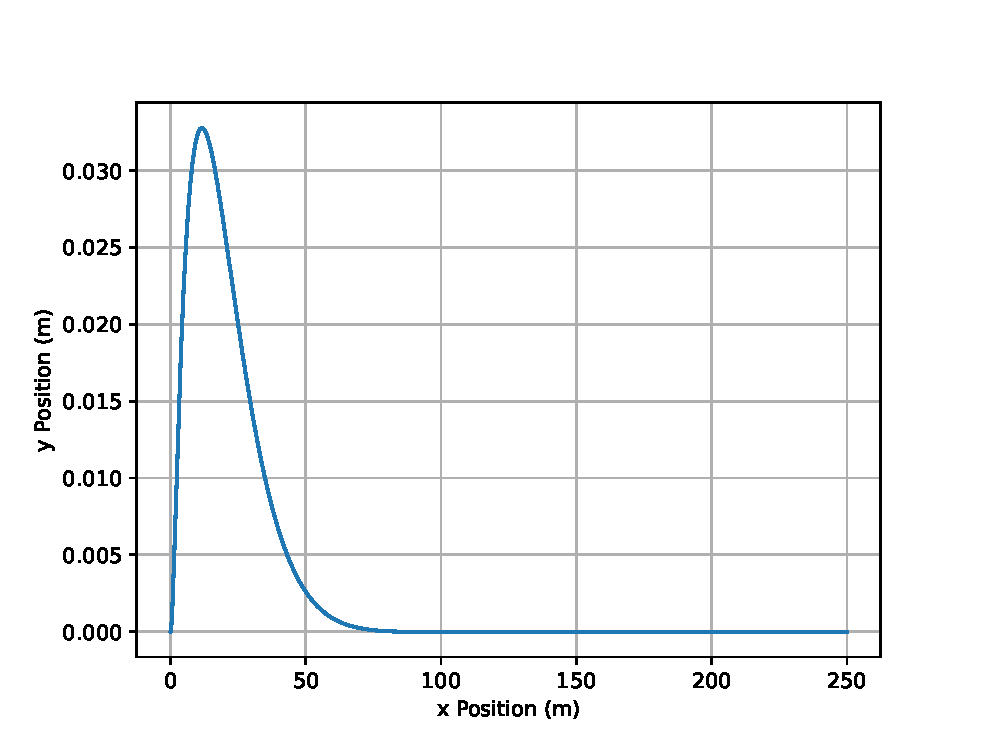
\includegraphics[width=0.6\linewidth]{figures/question_2_3_b.eps}
            \caption{A plot of the simulation of the vehicle with the y position of the vehicle in respect to the x position of the vehicle.}
        \end{figure}
        
        As \(K_i\) increases the steady equilibrium error of the system decreases. This reduces the effect of the additive disturbance. This will also reduce the stability of the system and increase the time taken for the vehicle to reach equilibrium.
        
    \subsection{Question 2.4}
        As sample rate is increased the rate of error correction done by the program also increases as the PID controller is only run every time the simulation is sampled. The integration step of the PID controller requires a sum of errors, however as this is only calculated when each sample is taken if there were a lower sampling time the system would take longer to account for any additive disturbances. It can therefore be concluded that a reduced sampling time is advantageous.


\end{document}
